\section{Antenna Basics}
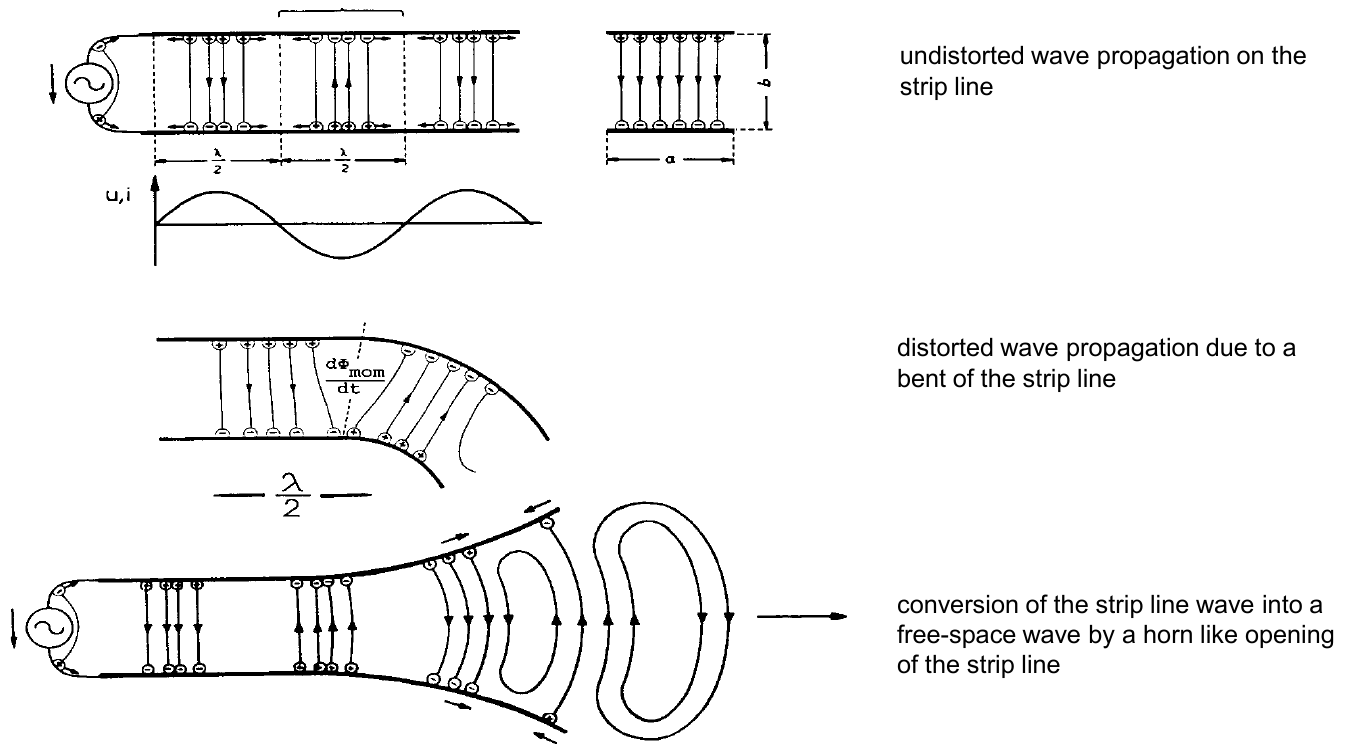
\includegraphics[width=.4\paperheight]{content/aawp/pictures/detachment_of_waves.png}
\begin{itemize}
    \itemsep0pt
    \item Input reflection coefficient:\\
        \[r \text{ or } \Gamma = S_{11} = \dfrac{Z - Z_0}{Z + Z_0} = -\dfrac{Y - Y_0}{Y + Y_0}\]
    \item Current and Voltage stop being useful for high frequencies\\
        $\implies$ Power wave amplitudes $a$ and $b$:
    \begin{align*}
        &a = \dfrac{U_{in} + I_{in}Z_0}{2\sqrt{Z_0}} & U_{in} = \sqrt{Z_0} (a + b)\\
        &b = \dfrac{U_{in} - I_{in}Z_0}{2\sqrt{Z_0}} & I_{in} = \dfrac{a - b}{\sqrt{Z_0}}
    \end{align*}
    \item Much like Current and Voltage, Impedance Matrices also stop making sense at higher frequencies\\
    $\implies$ Scattering matrix $S$:
        \[\begin{bmatrix}b_1\\ b_2\end{bmatrix} =\
            \begin{bmatrix}S_{11} & S_{12}\\ S_{21} & S_{22}\end{bmatrix} \
            \begin{bmatrix}a_1\\ a_2\end{bmatrix}\]
            \item \textbf{Symmetry:} \(\left(S = S^\top\right) \land \left(S_{ii} = S_{jj}\;\;\forall\:i, j \in \left[1;\:\mathrm{dim}\{S\}\right]\,\right)\)
    \item \textbf{Reciprocity:} \(S = S^\top\)
    \item There are 3 antenna field zones:
        \begin{enumerate}
            \itemsep0pt
            \item Reactive near-field
            \item Radiating near-field
            \item Far-field
        \end{enumerate}
    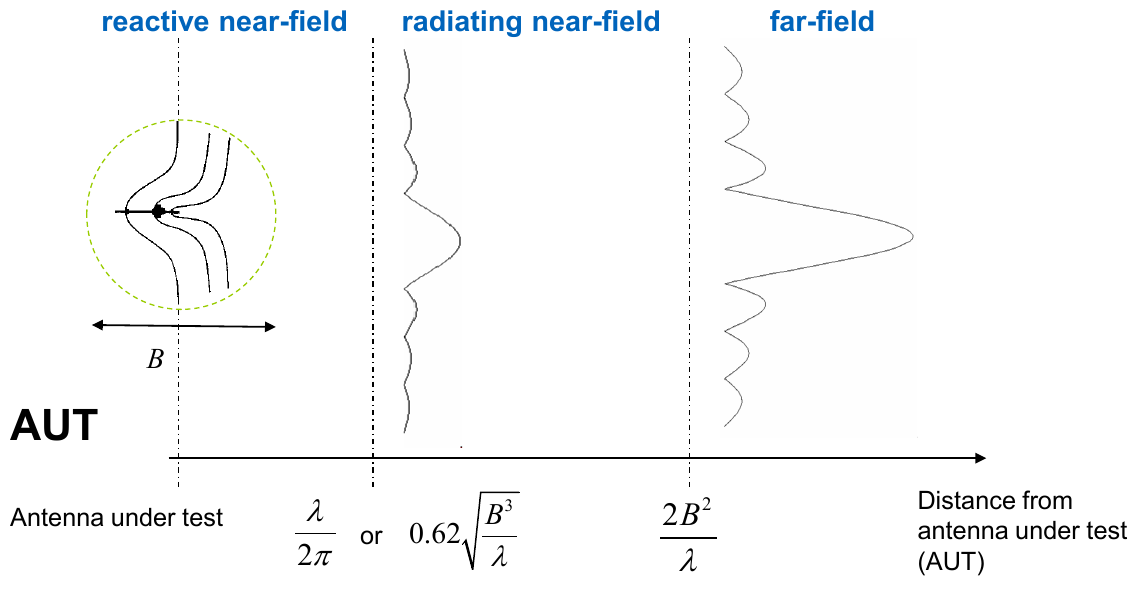
\includegraphics[width=.4\paperheight]{content/aawp/pictures/antenna_field_zones.png}
    \item Characteristics of the far-field:
        \begin{itemize}
            \itemsep0pt
            \item spherical wave fronts
            \item work with locally plane waves
            \item no reactive fields (\(\mathrm{Im}\{\vec{S}\} = 0\))
            \item \(|\vec{k}| = \omega \sqrt{\epsilon\mu}\), TEM-propagation
        \end{itemize}
    \item Poynting vectors: 
        \begin{align*}
            &\text{Far-field:} &S(r) = \dfrac{|E(r)|^2}{2 Z_{F0}},\;\; Z_{F0} \approx \SI{377}{\Omega}\\
            &\text{Reciprocal:} &S(r) = \dfrac{P_{t0}G_t}{4\pi r^2} = \dfrac{P_{t0}\eta D_t}{4\pi r^2}
        \end{align*}
    \item \textbf{Radiation Characteristic} $C(\vartheta, \varphi)$; angle-dependant antenna radiation under far-field conditions:
        \begin{equation*}
            C(\vartheta, \varphi) = \dfrac{E(\vartheta, \varphi)}{E_{max}}, \quad
            |C(\vartheta, \varphi)| = \sqrt{\dfrac{S(\vartheta, \varphi)}{S_{max}}}
        \end{equation*}
    \item Definitions of (Transmitted) Power:
        \begin{align*}
            &P_{t0} = (1- |\Gamma|^2) P_{t0,max},\text{ (Accepted)}\\
            &P_t = \eta_a P_{t0},\text{ (Radiated)}\\
            &P_t = \int\limits_{\vartheta=0}^{\pi} \int\limits_{\varphi=0}^{2\pi} S_{max} |C(\vartheta, \varphi)|^2 r^2 \sin(\vartheta)\: \mathrm{d}\vartheta \mathrm{d}\varphi\\
            &P_{t0,\mathrm{max}}\text{: Maximum (Generator) Power}
        \end{align*}
    \item Transmission Gain $G$ and Directivity $D$:
        \begin{align*}
            G_{(\mathrm{IEEE})} &= \left.\dfrac{S_{max}}{S_I}\right|_{P_{t0} = \mathrm{const}} &= \dfrac{S_{\mathrm{max}}}{P_{t0} / 4\pi r^2}\\
            D &= \left.\dfrac{S_{max}}{S_I}\right|_{P_{t} = \mathrm{const}} &= \dfrac{S_{\mathrm{max}}}{P_t / 4\pi r^2}
        \end{align*}
        \begin{equation*}
            G_{\mathrm{realized}} = (1 - |\Gamma|^2)G, \quad G = \eta D, \quad \eta = \dfrac{P_t}{P_{t0}}
        \end{equation*}
    \item Deriving \textit{directivity} D from Radiation Characteristic:\\
        \begin{align*}
            D &= \dfrac{4\pi}{\iint |C(\vartheta, \varphi)|^2 \sin(\vartheta) \mathrm{d}\vartheta\mathrm{d}\varphi}\\
            &= \dfrac{4\pi}{\Omega_a} \approx \dfrac{4\pi}{\varphi_{\SI{3}{dB}} \vartheta^\prime_{\SI{3}{dB}}}
        \end{align*}
    \item \textit{Effective area} $A_e$ and \textit{maximum effective area} (aperture) $A_0$ of reveiving antennas:\\
        \begin{align*}
            &A_e = \dfrac{P_{r,\mathrm{max}}}{S}\\
            &A_0 = \dfrac{P_{r0,\mathrm{max}}}{S}\\
            &P_{r0,\mathrm{max}}\text{: Maximum received power}
        \end{align*}
    \item For a \textit{reciprocal antenna} $\leftrightarrow$, the following holds:
        \begin{align*}
            A_0 &= \dfrac{\lambda_0^2}{4\pi} D &C_t(\vartheta, \varphi) = C_r(\vartheta, \varphi)\\
            A_e &= \dfrac{\lambda_0^2}{4\pi} G = \eta A_0&
        \end{align*}
    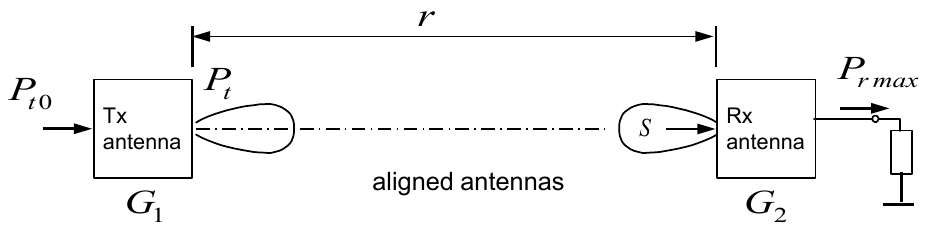
\includegraphics[width=.3\paperheight]{content/aawp/pictures/friis_transmission.png}
    \item \textbf{Friis Transmission Formula} for a radio link under far-field conditions:
        \begin{align*}
            &\dfrac{P_{r,max}}{P_{t0}} = G_1 G_2 \left(\dfrac{\lambda_0}{4\pi r} \right)^2,\\
            &r: \text{distance between antennas},\\
            &\lambda_0: \text{transmission wavelength},\\
            &G_1: \text{transmission antenna gain},\\
            &G_2: \text{receiving antenna gain}
        \end{align*}
    \item Radio Link Attenuation (\textit{Pathloss of free space}):\\
        \(\dfrac{a_0}{\si{dB}} = 10 \log_{10}^2\left(\dfrac{4 \pi r}{\lambda_0}\right) =\
        22 + 20 \log_{10}\left(\dfrac{r}{\lambda_0}\right)\)
\end{itemize}

\noindent\fbox{%
    \parbox{8cm}{%
        \textbf{How to Calculate Radiation Resistance} $R_r$:
        \begin{enumerate}
            \item Determine the antenna's current $I_a$ or its voltage $U_a$.
                \begin{equation*}
                    P_t = \dfrac{1}{2} |I_a|^2 R_r = \dfrac{1}{2} \dfrac{|U_a|^2}{R_r}
                \end{equation*}
            \item Equate the following with the above equation and solve for $R_r$:
                \begin{equation*}
                    P_t = \iint\limits_A \vec{S}(\vec{r}) \,\mathrm{d}\vec{A} = \iint\limits_A \dfrac{|E_{\mathrm{max}}|^2}{2 Z_F} |C(\vartheta,\varphi)|^2 \,\mathrm{d}\vec{A}
                \end{equation*}
        \end{enumerate}
    }}

%% Important definitions table:
\begin{tabular}{p{3cm}p{3.8cm}}
        \toprule
        IEEE Gain $G_{\mathrm{IEEE}}$ & How well the antenna converts the accepted power $P_{t0}$ into radiation in a certain direction for a lossy ($\eta<1$) antenna, and assuming perfect matching ($|\Gamma|^2 = 0$), which implies $P_{t0} = P_{t0,\mathrm{max}}$.\\\midrule
         Realized Gain $G$ & Less than the IEEE gain. Accepted power $P_{t0}$ is reduced by mismatch losses ($|\Gamma|^2 > 0$) of the antenna input impedance to a specified (reference) impedance. Power is reflected at the feed input.\\\midrule
        Maximum (Generator) Power $P_{t0,\mathrm{max}}$ & Generator power, assuming perfect matching ($|\Gamma|^2 = 0$) from the generator to the antenna.\\\midrule
        Accepted Power $P_{t0}$ & Power delivered from the generator via an antenna feed, assuming mismatching ($|\Gamma|^2 > 0$) from the feed to the antenna.\\\midrule
        Radiated Power $P_t$ & Power that is emitted as an EM-wave by an antenna after accounting for antenna ($\eta_a < 1$) and mismatching ($|\Gamma|^2 > 0$) losses.\\
        \bottomrule
\end{tabular}
